\documentclass[oneside, 11pt]{article}

\usepackage[T1]{fontenc}
\usepackage[utf8]{inputenc}
\usepackage[dutch]{babel}

\usepackage{fouriernc}
\usepackage[detect-all, load-configurations=binary,
            separate-uncertainty=true, per-mode=symbol,
            retain-explicit-plus, range-phrase={ tot }]{siunitx}

\usepackage{setspace}
\setstretch{1.2}

\setlength{\parskip}{\smallskipamount}
\setlength{\parindent}{0pt}

\usepackage{geometry}
\geometry{marginparwidth=0.5cm, verbose, a4paper, tmargin=3cm, bmargin=3cm, lmargin=2cm, rmargin=2cm}

\usepackage{float}

\usepackage[fleqn]{amsmath}
\numberwithin{equation}{section}
\numberwithin{figure}{section}

\usepackage{graphicx}
\graphicspath{{Figures/}}
\usepackage{subfig}

\usepackage{tikz}
\usetikzlibrary{plotmarks}

\usepackage{fancyhdr}
\pagestyle{fancy}
\fancyhf{}
\rhead{\thepage}
\renewcommand{\footrulewidth}{0pt}
\renewcommand{\headrulewidth}{0pt}

\usepackage{relsize}
\usepackage{xspace}
\usepackage{url}

\newcommand{\figref}[1]{Figuur~\ref{#1}}

\newcommand{\hisparc}{\textsmaller{HiSPARC}\xspace}
\newcommand{\kascade}{\textsmaller{KASCADE}\xspace}
\newcommand{\sapphire}{\textsmaller{SAPPHiRE}\xspace}
\newcommand{\jsparc}{\textsmaller{jSparc}\xspace}
\newcommand{\hdf}{\textsmaller{HDF5}\xspace}
\newcommand{\aires}{\textsmaller{AIRES}\xspace}
\newcommand{\csv}{\textsmaller{CSV}\xspace}
\newcommand{\python}{\textsmaller{PYTHON}\xspace}
\newcommand{\corsika}{\textsmaller{CORSIKA}\xspace}
\newcommand{\labview}{\textsmaller{LabVIEW}\xspace}
\newcommand{\daq}{\textsmaller{DAQ}\xspace}
\newcommand{\adc}{\textsmaller{ADC}\xspace}
\newcommand{\adcs}{\textsmaller{ADC}s\xspace}
\newcommand{\Adcs}{A\textsmaller{DC}s\xspace}
\newcommand{\hi}{\textsc{h i}\xspace}
\newcommand{\hii}{\textsc{h ii}\xspace}
\newcommand{\mip}{\textsmaller{MIP}\xspace}
\newcommand{\hisparcii}{\textsmaller{HiSPARC II}\xspace}
\newcommand{\hisparciii}{\textsmaller{HiSPARC III}\xspace}
\newcommand{\pmt}{\textsmaller{PMT}\xspace}
\newcommand{\pmts}{\textsmaller{PMT}s\xspace}

\DeclareSIUnit{\electronvolt}{\ensuremath{\mathrm{e\!\!\:V}}}

\DeclareSIUnit{\unitsigma}{\ensuremath{\sigma}}
\DeclareSIUnit{\mip}{\textsmaller{MIP}}
\DeclareSIUnit{\adc}{\textsmaller{ADC}}

\DeclareSIUnit{\gauss}{G}
\DeclareSIUnit{\parsec}{pc}
\DeclareSIUnit{\year}{yr}



\begin{document}

\title{Inregelen \pmts}
\author{D. B. R. A. Fokkema}
\date{}

\maketitle

\section{Werking van een \pmt}

Een fotoversterkbuis (photomultiplier tube, of \pmt) is een
elektronenbuis die in staat is om hele kleine lichtflitsjes om te zetten
in een elektrisch signaal.  Het is zelfs mogelijk om afzonderlijke fotonen
te tellen.  Geladen deeltjes uit kosmische straling die door de \hisparc
detectoren gaan verliezen energie in het materiaal van de detectoren.  In
de scintillator wordt dat energieverlies omgezet in een zwak
lichtschijnsel.  Dit paarsblauwe licht verspreidt zich door de detector
weerkaatst zo veel mogelijk aan de randen en een deel komt terecht bij de
\pmt, die het licht detecteert en een signaal afgeeft aan de \hisparc
elektronica.

Een \pmt maakt gebruik van het fotoelektrisch effect.  Dit effect werd
verklaard door Einstein en hiervoor ontving hij in 1921 de
Nobelprijs.\footnote{Veel mensen gaan er van uit dat Einstein de Nobelprijs
ontving voor de relativiteitstheorie, maar dit klopt niet.}  Wanneer licht
op een metaal schijnt, kunnen er elektronen worden losgeslagen uit het
oppervlak.  Dit gebeurt wanneer de energie per foton hoger is dan de
energie die een elektron nodig heeft om los te komen uit het metaal.  Deze
drempelenergie is afhankelijk van het soort metaal.  De energie per foton
wordt gegeven door
\begin{equation}
E_f = \frac{hc}{\lambda},
\end{equation}
met $E_f$ de energie van het foton, $h$ de constante van Planck, $c$ de
lichtsnelheid en $\lambda$ de golflengte van het licht.  Zie ook Tabel 7
en Tabel 35 in je Binas.

De energie van een foton is dus omgekeerd evenredig met de golflengte:
$E_f \propto 1/\lambda$.  Hoe kleiner de golflengte van het licht, hoe
groter de energie per foton.  Dit betekent dat hoe `blauwer' het licht,
hoe makkelijker een elektron wordt losgemaakt.  Is het licht \emph{te}
`rood', dan lukt dat nooit.  Daarom hebben we een scintillator gekozen die
een violet licht uitstraalt.

\begin{figure}
\centering
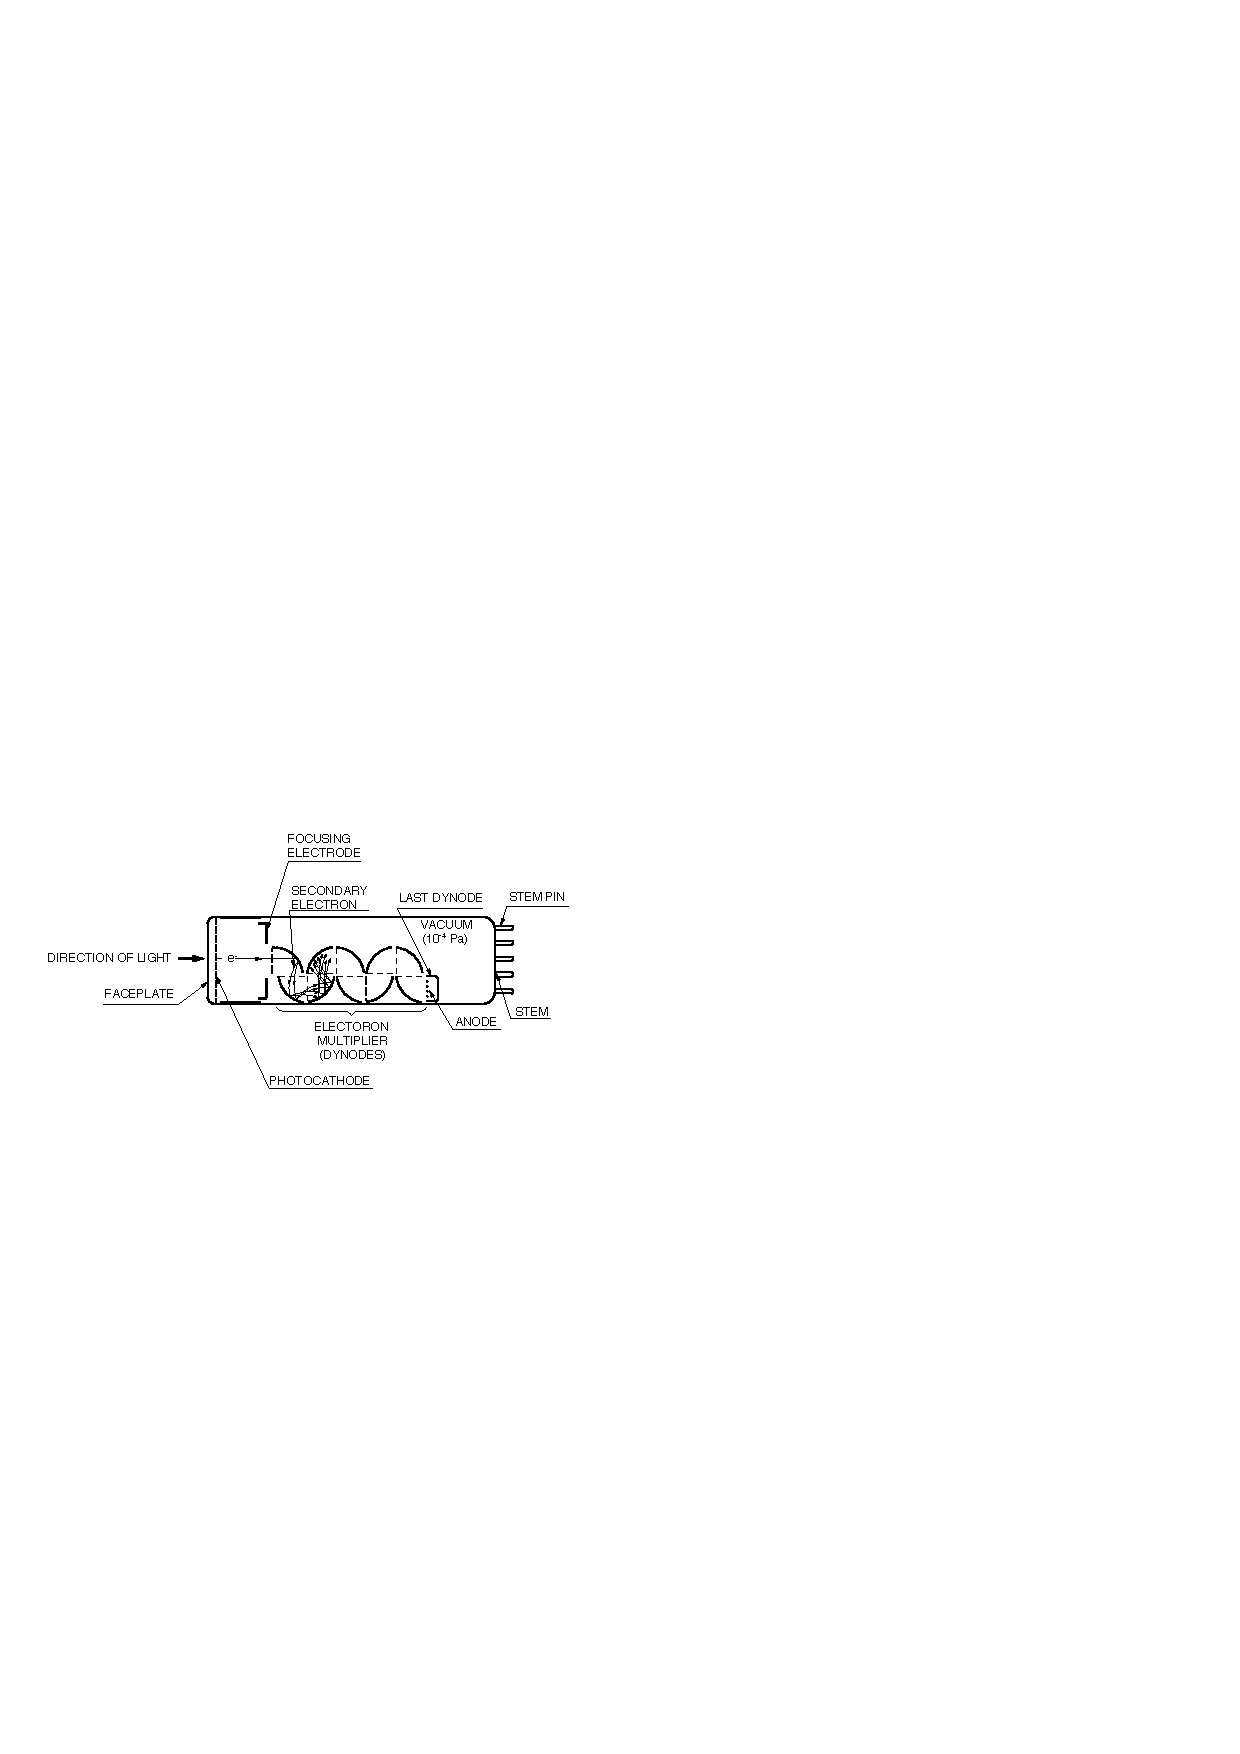
\includegraphics{pmt-schematic}
\caption{Schematische weergave van een \pmt.  Figuur overgenomen uit
\cite{hamamatsu}.}
\label{fig:pmt}
\end{figure}

De \pmt is een verzegelde glazen buis die vacuüm gemaakt
is\figref{fig:pmt}.  De voorkant van een \pmt bestaat uit een dunne
glaslaag.  Aan de binnenkant van het glas is een zeer dun metaallaagje
opgedampt.  Het laagje is zó dun, dat het doorzichtig is.  Licht dat op de
\pmt valt, gaat door het glas en raakt het metaal.  Het violette licht uit
de scintillator heeft een $E_f$ die hoog genoeg is om elektronen vrij te
maken uit het metaallaagje.  Om er voor te zorgen dat er veel elektronen
beschikbaar zijn wordt het metaalplaatje op een grote negatieve spanning
gezet.  De elektronen staan dan feitelijk te dringen om het metaal te
verlaten.  Het metaallaagje heet dan ook de \emph{kathode}\footnote{In een
vacuümbuis is de kathode de pool waar elektronen uit worden vrijgemaakt,
zoals hier gebeurt.} van de \pmt.  De \emph{anode} van de fotobuis wordt
geaard, waardoor er een sterk elektrisch veld in de buis ontstaat.  De
elektronen versnellen richting de anode.  Om een grote versterkingsfactor
te krijgen is de buis opgedeeld in meerdere trappen.  Iedere trap heeft
een \emph{dynode}, een metalen plaatje met een iets minder negatieve
spanning dan de voorgaande dynode.  Dus bij een \pmt met drie dynodes,
zijn de spanningen bijvoorbeeld als volgt: kathode (\SI{-1000}{\volt}),
eerste dynode (\SI{-750}{\volt}), tweede dynode (\SI{-500}{\volt}), derde
dynode (\SI{-250}{\volt}) en kathode (\SI{0}{\volt}).  Zo blijven de
elektronen versnellen van kathode, langs alle dynodes en uiteindelijk naar
de anode.  De versterking treedt op zodra de elektronen een dynode raken.
De grote snelheid waarmee een elektron het metaal intreedt maakt een
aantal elektronen los.  Deze losgeslagen elektronen worden vervolgens
versneld naar de volgende dynode.  Als per dynode per elektron
bijvoorbeeld drie elektronen worden losgeslagen, dan is de totale
versterking in een \pmt met tien dynodes gelijk aan $3^{10} \approx
\num{60000}$.  De hoogspanning die over de \pmt staat bepaalt in grote
mate de versterkingsfactor.  Hoe hoger de spanning, hoe groter de
versterkingsfactor.  De hoogspanning bepaalt namelijk enerzijds de
versnelling van de elektronen en anderzijds het aantal elektronen dat
staat te dringen om de dynode te verlaten.

De \pmt die gebruikt wordt door \hisparc is een 9107B van Electron
Tubes \cite{9107B}.  Deze heeft 11 dynodes en een typische versterking van
\num{3e6} bij \SI{850}{\volt}.  Dat komt overeen met $\num{3.9}^{11}$.  Voor
ieder elektron dat een dynode raakt worden er gemiddeld bijna vier
elektronen vrijgemaakt.


\section{Signaal uit \hisparc detectoren}
\subsection{Pulshoogtehistogram}
\subsection{Drempels}

\section{Inregelen \pmts}


\begin{thebibliography}{9}
\bibitem{hamamatsu} Hamamatsu, \emph{Photomultiplier Tubes, Construction
and Operating Characteristics Connections to External Circuits} (1997).
\bibitem{9107B} ET Enterprises, Ltd., \emph{9107B series data sheet}
(2010), \url{http://my.et-enterprises.com/pdf/9107B.pdf}.
\end{thebibliography}

\end{document}
